\chapter{Metodología: Clásica VS Ágil}

El primer aspecto a tener en cuenta al inicio de un proyecto, es la elección de la metodología de gestión del proyecto. En principio podemos distinguir dos grupos de metodologías: clásica y ágil.

\section{Tipos de metodologías}

\subsection*{Metodología Clásica}

La metodología clásica se caracteriza por una estructura secuencial y un flujo de proceso lineal. La metodología clásica lleva consigo décadas de recopilación de experiencias previas en proyectos. Aunque viendo su nombre parezca que se trata de una metodología arcaica y en desuso, no es así bajo ningún concepto. Esta metodología se sigue puliendo y mejorando actualmente, aunque uno de sus problemas es su enfoque ``mayorista'', es decir, la metodología está enfocada a los macro-proyectos. Un macro-proyecto es un proyecto con una gran inversión y con un equipo de trabajo de varias decenas de personas, con los roles bien definidos. Aunque un proyecto no encaje con la definición de macro-proyecto, esta metodología se puede adaptar al proyecto en cuestión.

La metodología clásica o metodología ``en cascada'' está definida por las siguientes etapas:

\begin{figure}[h]
    \centering
    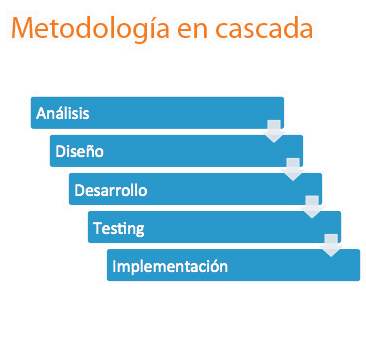
\includegraphics[width=0.6\textwidth]{imagenes/metodologia/meto_clasica.jpg}
    \caption{Etapas de la metodología clásica}
\end{figure}

\newpage

Dado que la metodología clásica sólo consta de un ciclo para realizar las etapas, será imprescindible una buena planificación de alcance, tiempo y coste del proyecto y de cada una de las etapas. Esta planificación inicial es tan importante porque no se obtendrán resultados del proyecto hasta que se encuentre cercano a su cierre.

Entre los problemas de la metodología clásica podemos encontrar los siguientes:

\begin{itemize}
    \item Los proyectos reales difícilmente se adecuan a este modelo de proceso.
    \item Dificultad para expresar por parte del cliente todos los requisitos al principio del proyecto.
    \item Poca comunicación con cliente/usuario, hasta las etapas finales no hay un ejecutable que se pueda evaluar.
\end{itemize}

\subsection*{Metodología Ágil}

La metodología ágil se caracteriza por una estructura incremental y un flujo de proceso iterativo. Esta metodología surge como solución a los problemas de la metodología clásica, sobretodo en la planificación de proyectos cortos y cambiantes. Esta metodología se adapta mejor a los proyectos del ámbito de las TIC, es decir, en el desarrollo de software. Esto es debido a que la metodología ágil consiste en la realización de continuas iteraciones, donde cada iteración da como resultado un prototipo del proyecto. Este modo de trabajar no se adecua a proyecto que puedan estar relacionados con el sector de la construcción, como puede ser la construcción de un puente, dado que no se pueden crear prototipos de una construcción ya que no serían seguros, y además son proyectos poco cambiantes en los requisitos del proyecto durante su desarrollo.

La metodología ágil está definida por las siguientes etapas:

\begin{figure}[h]
    \centering
    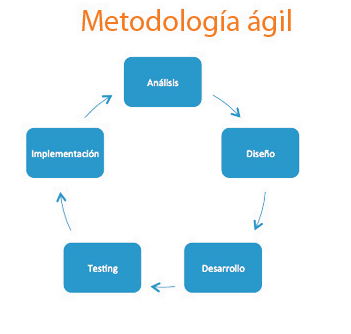
\includegraphics[width=0.6\textwidth]{imagenes/metodologia/meto_agil.jpg}
    \caption{Etapas de la metodología ágil}
\end{figure}

\section{Elección de la metodología}

La metodología que seguiré para el desarrollo de mi TFG es la metodología ágil. Pienso que es la metodología que más se adecua a las condiciones de mi proyecto, dado el limitado tiempo y la multitud de cambios que surgirán durante el desarrollo del mismo. Además la creación de prototipos ayudará a la mejora incremental de las funcionalidades del proyecto, teniendo en todo momento al menos un prototipo funcional que se pueda evaluar tanto por parte del tutor como del tribunal.